%Chapter 5


% -- not sure if this is Kosher -- removes double space before eq'ns
\makeatletter
\def\env@matrix{\hskip -\arraycolsep
  \let\@ifnextchar\new@ifnextchar
  \linespread{1}\selectfont
  \renewcommand{\arraystretch}{0.5}%
  \array{*\c@MaxMatrixCols c}}
\makeatother


\renewcommand{\thechapter}{5}

\chapter{Quasi-integrable Octupole Lattice}

As introduced in Chapter 1, a quasi-integrable octupole lattice is proposed as a way to mitigate space charge in accelerator rings. Large amplitude-dependent tune spreads, driven by strong nonlinear magnet inserts, lead to decoupling from incoherent tune resonances. This reduces intensity-driven beam loss while quasi-integrability ensures a well-contained beam. In this chapter I discuss on-going work to install and interrogate a long-octupole channel at UMER, as well as explore simulated properties of the proposed nonlinear lattice. This is a discrete insert that occupies 20 degrees of the ring, consisting of independently powered printed circuit octupole magnets. Transverse confinement is obtained with quadrupoles external to this insert. Operating UMER as a non-FODO lattice, in order to meet the beam-envelope requirements of the quasi-integrable lattice, is a challenge. 





%%%%%%%%%%%%%%%%%%%%%%%%%%%%%%%%%%%%%%%%%%%%%%%%%%%%%%%%%%%%%%%%%%%%%%%%%%%%%%%%%%%%%%%%%%%%%%%%%%%%%%%%%%%%%%%%%%%%%%%

\section{Nonlinear UMER lattice}

\begin{figure}
\centering
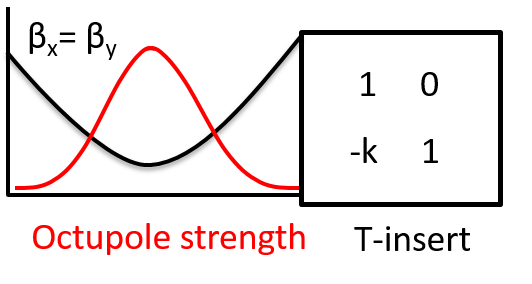
\includegraphics[width=.5\textwidth]{gen.figures/toy_model.png}
\caption{Simple quasi-integrable system: FOFO focusing with nonlinear insert }
\label{fig:toymodel}
\end{figure}

\begin{figure}[]
\centering
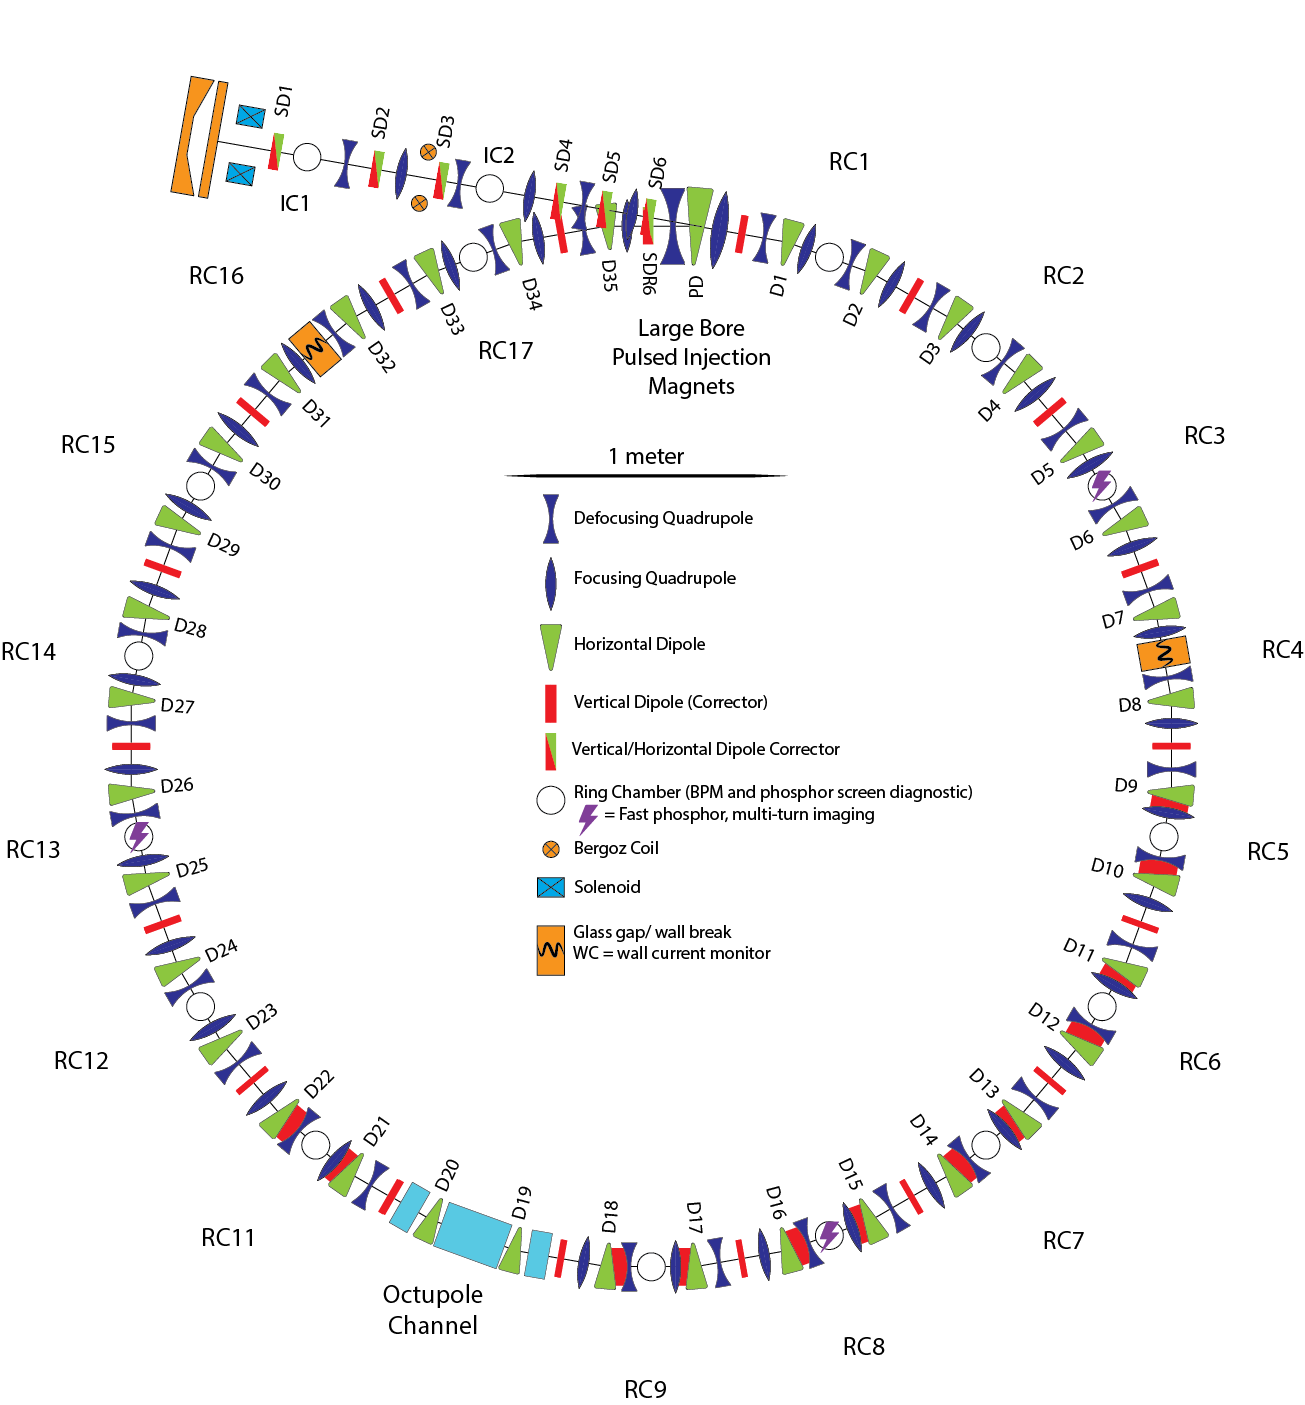
\includegraphics[width=\textwidth]{umer-diagram/full_octu_ring.png}   
\caption{UMER lattice with planned future octupole channel (light blue elements at RC10 location).}
\label{fig:octring}
\end{figure}  


The theory of quasi-integrable nonlinear optics assumes a symmetric beam is propagating in nonlinear fields that are scaled longitudinally with the inverse of the envelope function. External linear focusing must be provided for a bounded envelope function. 
To achieve this in a ring, a nonlinear channel is installed over a symmetric beam waist, and a linear lattice insert,
with a transfer function equivalent to a thin, x-y symmetric focusing lens, images the beam from the exit to the entrance of the channel. This is shown schematically in Fig. \ref{toymodel}.

To modify UMER as a nonlinear optics test bed, we will superimpose an octupole channel onto the existing lattice, as shown in fig. \ref{fig:octring}.
Printed circuit octupole magnets will share magnet mounts with existing printed circuit quadrupoles, over a fraction ($32 - 64$ cm) of the ring. 
The surrounding quadrupole lattice will act as an effective $0 \cdot \pi$ thin lens transfer matrix, by independently varying the strengths of the quadrupoles in the ring to attain the proper transfer function. 
A linear lattice solution for the nonlinear UMER ring can be found in \cite{AAC}, although this solution is not optimized for large tune spread.








\section{Simple Quasi-integrable Simulation Model}

The prescription for a strongly nonlinear lattice with 1 or 2 analytic invariants is laid out in Danilov and Nagatisev's 2010 publication \cite{Danilov2010}.

We first model an ideal quasi-integrable octupole channel, in which octupoles are perfectly scaled as $\beta^{-3}$ across a 64 cm drift (equivalent 20 degree section of UMER), and the remaining 340 degrees of the ring is condensed to a thin-lens axisymmetric focusing kick. This system is discussed in more detail in previous presentations \cite{KRAAC}.

%%%%%%%%%%%%%%%%%%%%%%%%%%%%%%%%%%%%%%%%%%%%%%%%%%%%%%%%%%%%%%%%%%%%%%%%%%%%%%%%%%%%%%%%%%%%%%%%%%%%%%%%%%%%%%%%%%%%%%%%%%
%% from AAC14
%%%%%%%%%%%%%%%%%%%%%%%%%%%%%%%%%%%%%%%%%%%%%%%%%%%%%%%%%%%%%%%%%%%%%%%%%%%%%%%%%%%%%%%%%%%%%%%%%%%%%%%%%%%%%%%%%%%%%%%%%%
WARP PIC simulations have been used to predict octupole lattice behavior. Preliminary simulations have been limited to a 2D transverse geometry “toy-model” of the system, consisting of a 32 cm channel with longitudinally varying octupole fields alternating with an X-Y symmetric thin lens kick, which approximates the linear section of the ring. Figure 3 shows a schematic of the PIC simulation setup.

\subsection{Invariant tracking in simple quasi-integrable lattice.}

We use the WARP PIC code to track the invariant quantity (Hamiltonian) in the nonlinear lattice \cite{warp}. 

For 100 passes through this octupole channel, we see a particle of $\langle H_N\rangle =1E-5$ experience RMS variations of $2.8E-10$ without octupoles (jitter apparently due to computational noise) and variations of $1.5E-8$ for maximum octupole current of 2 A. These values can be compared to Table \ref{l2ea4-t1}. Despite low-frequency oscillations, the particle energy appears to be well-bounded as expected, see Fig. \ref{toyinvar}.

\begin{figure}[]
   \centering
    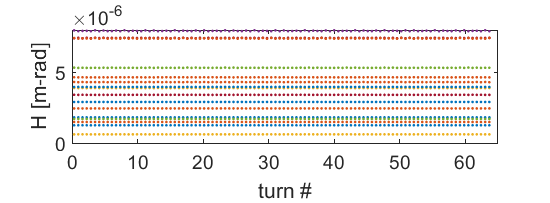
\includegraphics[width=0.5\textwidth]{5.figures/HvsZ_crun1_toylattice.png}
 	\caption{Conserved invariant $H_N$ for simple quasi-integrable octupole lattice, WARP simulation}
   \label{toyinvar}
\end{figure}



\subsection{Frequency Map Analysis of Chaotic Octupole Lattice}

%todo: Cover WARP and Elegant models, estimate tune prediction

\subsection{Choosing Octupole Operating Point}

\begin{figure}[]
\centering
\subfigure[]{
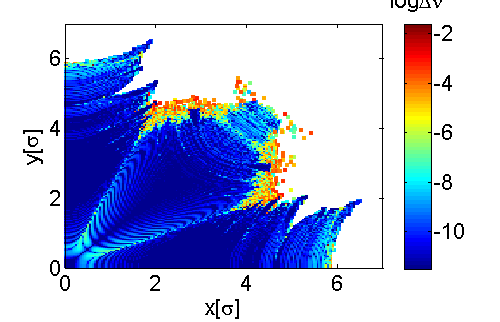
\includegraphics[width=0.35\textwidth]{5.figures/FMA/WARP_fma_nu087.png}
\label{fig:toy-fma-configspace}
}
\hspace{.5in}
\subfigure[]{
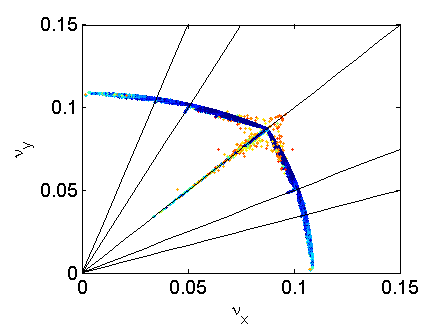
\includegraphics[width=0.35\textwidth]{5.figures/FMA/WARP_fma_nu087_tunespace_reslines.png}
\label{fig:toy-fma-tunespace}
}
\caption{Frequency map analysis (FMA) of toy octupole lattice in WARP PIC code. (a) Change in tune vs. particle launch position. (b) Tune footprint, with 1st to 3rd order resonances.}
\label{fig:toy-fma}
\end{figure}

\begin{figure}[]
\centering
\subfigure[]{
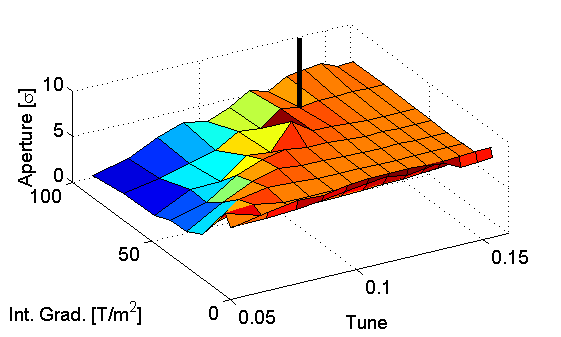
\includegraphics[width=0.4\textwidth]{5.figures/FMA/parameter_scan_aperture.png}
\label{fig:fma-op-aperture}
}\hspace{.25in}
\subfigure[]{
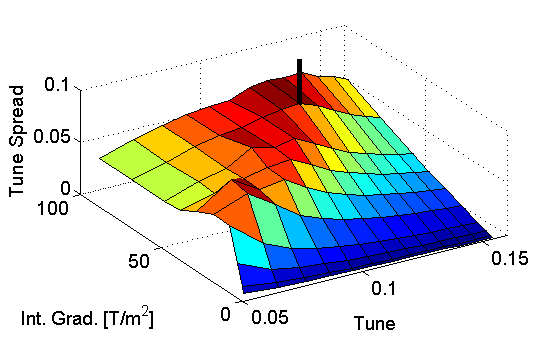
\includegraphics[width=0.4\textwidth]{5.figures/FMA/parameter_scan_tunespread.png}
\label{fig:fma-op-tune}
}
\caption{Parameter space landscape of toy octupole lattice, generated with Elegant FMA for 1024 turns. (a) Dynamic aperture and (b) Maximum tunespread vs. integrated octupole strength and lattice tune.}
\label{fig:fma-op}
\end{figure}



%%%%%%%%%%%%%%%%%%%%%%%%%%%%%%%%%%%%%%%%%%%%%%%%%%%%%%%%
The maximum achievable tune spread depends on the phase advance through the nonlinear channel and the octupole strength.
 

Fig. \ref{fig:toy-fma} shows the frequency map for a 'toy model' of the UMER octupole lattice. 10 keV electrons pass through an ideal octupole channel (no fringe fields), and the linear part of the lattice is condensed into a thin, 0-phase advance, X-Y symmetric focusing 'kick.'
This map is generated with single particle tracking through an ideal lattice in the WARP PIC code \cite{warp} with no space charge. 
The fractional tune of the lattice is relatively low ($\nu = 0.087$) and maximum possible tune spread is predicted to be 0.10 in WARP and 0.06 in Elegant. 



The FMA plots show that the regions of large octupole-induced tune shifts are close to the limit of acceptance, making it ideal to operate with a dynamic aperture within several beam sigmas. 
Fig. \ref{fig:fma-op} shows the landscape of the toy model in lattice tune/octupole strength parameter space as simulated in Elegant. 
The plateau on fig. \ref{fig:fma-op-aperture} is an artifact of the simulation size (7 beam sigmas). Without this artificial limit, aperture increases with decreased field strength, until limited by the beam pipe.

It is apparent that, while the octupole tune shift increases with octupole strength, the dynamic aperture decreases. 
The maximum octupole strength also increases with phase advance in the channel, as $\max{\left( K_3(s)\right)} \propto \max{\left(\frac{1}{\beta(s)^3}\right)}$ increases. 
The vertical marker in fig. \ref{fig:fma-op} indicates the best operating point for the parameter space that was investigated. 
At a fractional tune of $\nu = 0.12$ and integrated octupole gradient of $15$  $\frac{T}{m^2}$, the absolute maximum tune spread is $0.08$. 
This octupole strength corresponds with a peak strength of $54$  $\frac{T}{m^3}$, which is easily attainable for printed circuit octupoles, as explained below.

Based on the shape of the parameter landscape, it is desirable to push towards higher tunes and larger octupole gradients for larger tune spreads, ideally $> 0.10$.


\subsection{Phase Advance in UMER}

The maximum phase advance will be limited by the available focusing strength in the linear lattice.
0-current envelope tracking in Elegant show how the UMER lattice can be modified to imitate a 0-phase advance focusing lens.\cite{RuisardAAC2014} 
Phase advance of $0.087$ has been demonstrated using 14 quadrupoles to match a 32 cm octupole channel with a FODO lattice. Greater phase advance is possible, but 
the maximum phase advance in the octupole channel is limited by the allowable excursion of the envelope ($\leq1$ meter).

Solenoids are considered for the matching section, to increase the attainable phase advance through the octupole channel. 
With solenoids, phase advance of $0.4\cdot2 \pi$ was obtained in a 32 cm drift. 
While the increase in phase advance (and therefore tune spread) is dramatic, use of solenoids creates additional alignment challenges. 
%%%%%%%%%%%%%%%%%%%%%%%%%%%%%%%%%%%%%%%%%%%%%%%%%%%%%%%%%%%%%%%%%%%%%%%%%%%%%%%%%%%%%%%%%%%%%%%%%%%%%%%%%%%%%%%%%%%%%%%



























\subsection{Steering Tolerances}

The effect of background fields on the low-rigidity UMER beam is significant.  The vertical field is almost constant at all ring sections at an average of 400 mG for approximately 2.2° of bend angle per horizontal dipole. The radial field has a sinusoidal variation with amplitude 200 mG, for maximum bend angle of 2.2° per vertical corrector. Therefore, the closed orbit will not be perfectly aligned to element centers, but rather lie within an acheivable tolerance. Additionally, the closed orbit is necessarily not straight but arcs between corrector magnets. Finally, the beam centroid will not perfectly follow the closed orbit, but oscillates about it at the betatron frequency. 

To consider the effect of imperfect orbit correction on particle stability in the quasi-integrable octupole lattice, I apply frequency map analysis and examine dynamic aperture and maximum tune spread. I consider distortions of closed orbit, but oscillations about closed orbit. I also do not consider mis-alignment of octupole elements in the channel. A gross mis-alignment of the long-channel mount can be considered equivalent to an orbit distortion, while misalignments between individual circuits in the long channel require different treatment.

Tolerance simulations use the WARP PIC code to model a 64 cm octupole channel with an ideal linear FOFO thin-lens transformation. In the simulation, a constant closed orbit distortion term is included in the trajectory calculations for each particle as thin lens transformations. Two cases are examined:

\begin{enumerate}
\item Orbit distortion in otherwise shielded 64 cm section (centroid has straight trajectory between steering elements.)
\item Curved orbit distortion due to constant background field
\end{enumerate}

\subsubsection{Case 1: Straight/shielded orbit distortion}

\begin{figure}
\centering
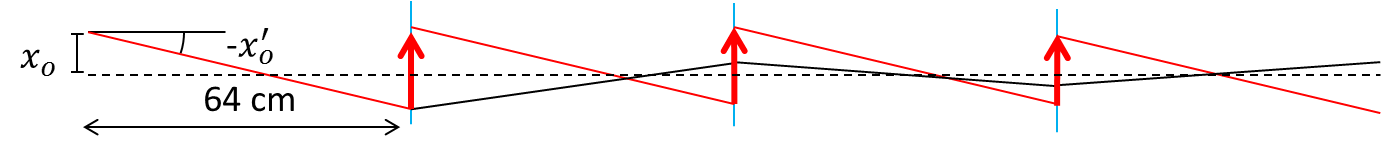
\includegraphics[width=\textwidth]{5.figures/steeringtolerance/orbit_distortion_cartoon.png}
\caption{Red line is centroid motion of beam with initial offset $x_0$, $x'_0$. Thick red lins indicate thin lens centroid transformation. Black line is centroid motion without centroid transformation.}
\label{fig:straightorbitdistortion}
\end{figure}

Fig. \ref{fig:straightorbitdistortion} shows distortion of the closed orbit in the case where particle trajectories are straight between magnetic elements (. The distortion is defined by initial conditions $x_0$ and $x'_0$. At the same location as the FOFO thin lens transformation (that represents focusing in the linear part of the ring), a centroid transformation is also made. For a single plane,

\begin{equation}
\begin{bmatrix} x \\ x' \end{bmatrix}_f = \begin{bmatrix} x \\ x' \end{bmatrix}_i + \begin{bmatrix} -L x_0 \\ k(x_0 + Lx_0') \end{bmatrix}
\label{eq:straightorbitdistortion}
\end{equation}

The derivation follows. Consider single particle matrix equations for propagation through a focusing element (strength $k$) and a drift of length $L$. 

\begin{equation}
\begin{split}
\begin{bmatrix} x \\ x' \end{bmatrix}_f 
& = \begin{bmatrix} 1&0 \\ -k&1 \end{bmatrix}_i \ast \begin{bmatrix} 1&L \\ 0&1 \end{bmatrix}_i \ast \begin{bmatrix} x \\ x' \end{bmatrix}_i \\
& = \begin{bmatrix} x_i + Lx'_i \\ -kx_i + (1-kL)x'_i \end{bmatrix}
\end{split}
\end{equation}

Now divide motion into single particle $x_p$ and centroid $x_c$ components, where $x_i = x_{c,i} + x_{p,i}$ and $x'_i = x'_{c,i} + x'_{p,i}$. The matrix equation for a single pass becomes:

\begin{equation}
\begin{split}
\begin{bmatrix} x \\ x' \end{bmatrix}_f 
&= \begin{bmatrix} x_{c,i} + Lx'_{c,i} \\ -kx_{c,i} + (1-kL)x'_{c,i} \end{bmatrix} + \begin{bmatrix} x_{p,i} + Lx'_{p,i} \\ -kx_{p,i} + (1-kL)x'_{p,i} \end{bmatrix} \\
&=\begin{bmatrix} x_p \\ x'_p \end{bmatrix}_f + \begin{bmatrix} x_c \\ x'_c \end{bmatrix}_i + \begin{bmatrix} L x_{c,i} \\ -k(x_{c,i} + Lx'_{c,i}) \end{bmatrix}
\end{split}
\end{equation}

Considering $\begin{bmatrix} x \\ x' \end{bmatrix}_f = \begin{bmatrix} x_c \\ x'_c \end{bmatrix}_f + \begin{bmatrix} x_p \\ x'_p \end{bmatrix}_f$, one can examine just the centroid motion $\begin{bmatrix} x_c \\ x'_c \end{bmatrix}_f = \begin{bmatrix} x_c \\ x'_c \end{bmatrix}_i + \begin{bmatrix} L x_{c,i} \\ k(x_{c,i} + Lx'_{c,i}) \end{bmatrix}$. Let $x_{c,i} = x_0$ and $x'_{c,i} = x'_0$. The centroid will propogate identically through the 64 cm channel from turn to turn if $\begin{bmatrix} L x_0 \\ -k(x_0 + Lx_0') \end{bmatrix}$ is subtracted at the end of each pass, as in Eq. \ref{eq:straightorbitdistortion}.

It should be noted that in case 1, I ignore the effect of the bending dipoles, which are spaced at 32 cm intervals. This is palatable under two assumptions: the bending dipole field is "flat" (bend angle does not depend on displacement in dipole) and, in a shielded environment, there is a setting for the dipoles that allows the beam to propogate centered through all elements. 

\begin{figure}
\centering
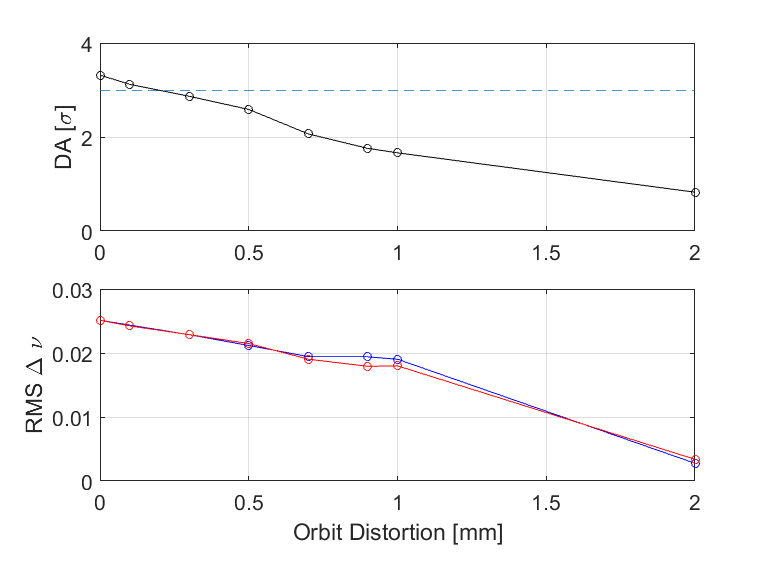
\includegraphics[width=0.8 \textwidth]{5.figures/steeringtolerance/DA_deltanu_plots_vs_orbit_distortion.png}
\caption{Dependence of dynamic aperture and tune spread on orbit distortion. On dynamic aperture (DA) plot, horizontal dashed line indicates $90\%$ of ideal aperture.}
\label{fig:DAvsorbitdistort}
\end{figure}

While $x_0$, $x'_0$ is a two-dimensional space of possible orbit distortion, I simplified the problem by requiring that the distortion be symmetric in a 64 cm drift. That is, $x_f = -x_0$ and $<x(s)> = 0$. In this case, $x'_0 \approx \sin{x'_0} = L/2x_0$ and the distortion is parametrized in terms of $x_0$ only. For a range of distortions $x_0$, I run the WARP simulation and apply FMA. Octupole strength is parametrized by peak strength in the channel, set at $50 T/m^3$ for these simulations, which is approximately $1 A$ excitation for the physical coils. 
 
I assume a round beam in the channel. As the dynamic aperture is not round, in this case I quantify radial dynamic aperture as the largest radius circle for which no particles are lost. Fig. \ref{fig:DAvsorbitdistort} shows the results from multiple dynamic aperture calculations. There is quite a stringent requirement on distortion, with $x_0 < 0.2$ mm desired for preservation of dynamic aperture. At $x_0 = 0.2$ mm, decrease of RMS tune spread from ideal case of 0.025 is $\approx 6\%$.




\subsubsection{Case 2: Curved orbit distortion due to background field}

\begin{figure}
\centering
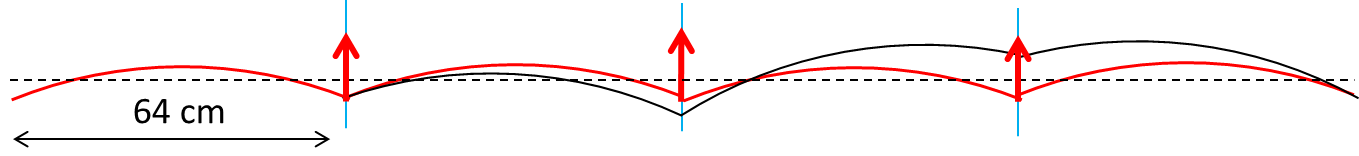
\includegraphics[width=\textwidth]{5.figures/steeringtolerance/vert_bg_field_distortion_cartoon.png}
\caption{Red line is centroid motion of beam with thin lens centroid transformation at thick red arrows. Black line is centroid motion without centroid transformation, just periodic thin lens focusing element.}
\label{fig:vertcurvedorbitdistortion}
\end{figure}

To model the effect of orbit  due to immersion in ambient background fields, I applied a similar thin-lens centroid transformation. Fig. \ref{fig:vertcurvedorbitdistortion} shows the case where steering corrections are made every 64 cm, which represents vertical steering with RSV steerers. The orbit is assumed to be "as centered as possible." For a given background field, initial conditions $y_0$ and $y'_0$ are chosen so that $y_i=y_f$ across a 64 cm drift, and $\max{y}=\min{y}$ in the drift. In this case, the centroid correction is simply:

\begin{equation}
\begin{bmatrix} y \\ y' \end{bmatrix}_f = \begin{bmatrix} y \\ y' \end{bmatrix}_i + \begin{bmatrix} 0 \\ ky_0 + \theta \end{bmatrix}
\label{eq:curvedorbitdistortion}
\end{equation}

$\theta$ is the bending angle due to the background field. Assuming a constant background field, $\theta = \frac{LB_x}{B \rho}$ depends only on channel length (64 cm), background field $B_x$ and particle rigidity $B \rho$. To meet the condition $y_i=y_f$, $y'_0 = \theta/2$. To satisfy $\max{y}=\min{y}$, $y_0=\rho/2 \cdot ( 1-\cos{(\theta/2)} )$.    

\begin{figure}
\centering
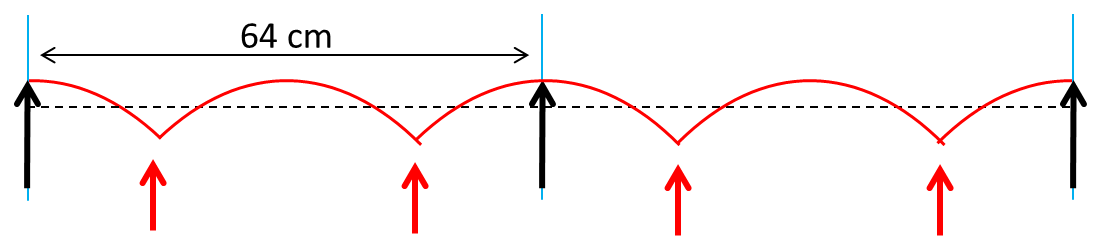
\includegraphics[width=\textwidth]{5.figures/steeringtolerance/horz_bg_field_distortion_cartoon.png}
\caption{Red line is centroid motion of beam with thin lens centroid transformation at thick red arrows. Thick black arrows indicate thin-lens focusing element.}
\label{fig:horzcurvedorbitdistortion}
\end{figure}

As horizontal steerers are located every 32 cm and will be co-housed in the long 64-cm octupole channel, a slightly different transformation is applied for the case of horizontal steering. The steering correction of Eq. \ref{eq:curvedorbitdistortion} is split and applied at different locations: 

\begin{subequations}
\begin{equation}
\begin{bmatrix} x \\ x' \end{bmatrix}_f = \begin{bmatrix} x \\ x' \end{bmatrix}_i + \begin{bmatrix} 0 \\ kx_0 \end{bmatrix}
\label{eq:horzcurvedorbitdistortion1}
\end{equation}
\begin{equation}
\begin{bmatrix} x \\ x' \end{bmatrix}_f = \begin{bmatrix} x \\ x' \end{bmatrix}_i + \begin{bmatrix} 0 \\ \theta \end{bmatrix}
\label{eq:horzcurvedorbitdistortion2}
\end{equation}
\end{subequations}

\begin{figure}
\centering
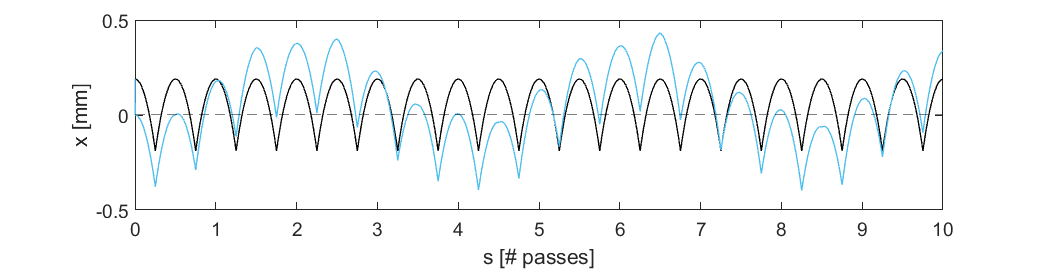
\includegraphics[width=\textwidth]{5.figures/steeringtolerance/sp_traces.png}
\caption{Particle tracing results showing particle launched on closed orbit (black) and particle with initial offset (blue) in horizontal plan. Octupole fields are turned off.}
\label{fig:horsptraces}
\end{figure}

Eq. \ref{eq:horzcurvedorbitdistortion1} is applied at the ends of the 64 cm channel, same location as the thin-lens focusing kick, essentially cancelling the effect of thin lens focusing on the centroid. Eq. \ref{eq:horzcurvedorbitdistortion1} is applied every 32 cm at dipole locations (in 64 cm channel, at $s=16,48$ cm). This is pictured in Fig. \ref{fig:horzcurvedorbitdistortion}. Fig. \ref{fig:horsptraces} shows resulting orbits over 10 passes through a 64 cm drift. No steering compensation is made when octupole fields are included.

\begin{figure}
\centering
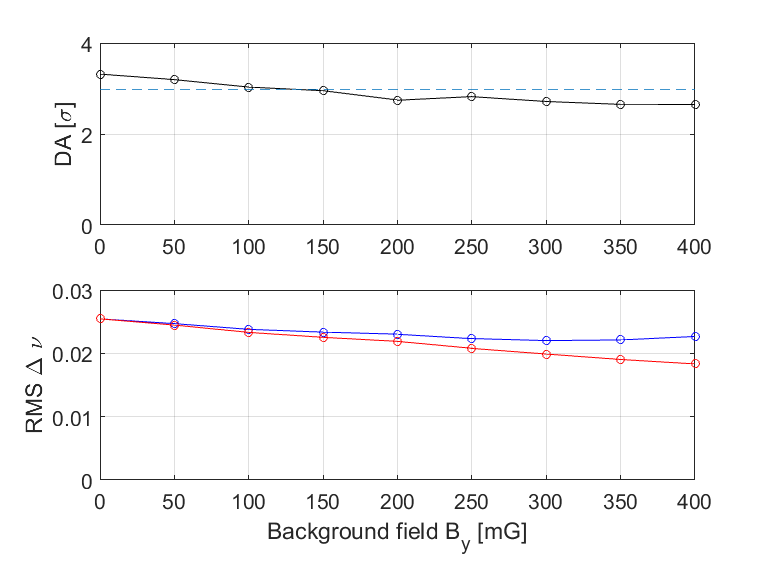
\includegraphics[width=0.8\textwidth]{5.figures/steeringtolerance/DA_deltanu_plots_vs_background_By.png}
\caption{Dependence of dynamic aperture and tune spread on vertical background field. On dynamic aperture (DA) plot, horizontal dashed line indicates $90\%$ of ideal aperture.}
\label{fig:DAvsBGfield}
\end{figure}

\begin{figure}
\centering
\subfigure[Dynamic aperture contours for beam immersed in vertical field, Max. Octupole strength $50 T/m^3$.]{
	\centering
	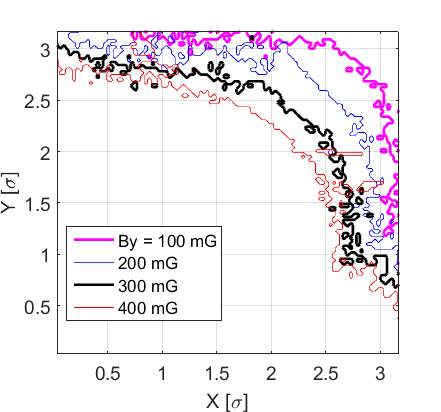
\includegraphics[width=0.45\linewidth]{5.figures/steeringtolerance/FMA_007_DAcontours.png}
	}
	\label{fig:FMADA1}
\hfill
\subfigure[Dynamic aperture contours for beam immersed in vertical and horizontal fields, Max. Octupole strength $50 T/m^3$.]{
	\centering
	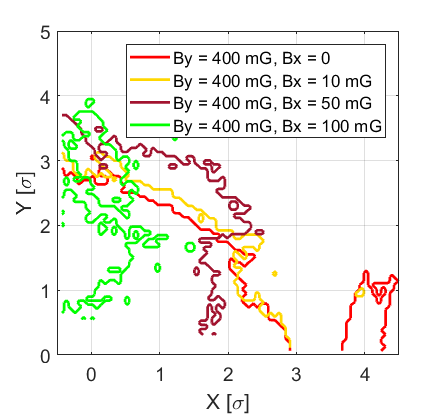
\includegraphics[width=0.45\linewidth]{5.figures/steeringtolerance/FMA_009_DAcontours.png}
	}
	\label{fig:FMADA2}
\end{figure}


In Fig. \ref{fig:DAvsBGfield} and Fig. \ref{fig:FMADA1} we see that the presence of a vertical background field, there is an $80\%$ loss of radial dynamic aperture at 400 mG when compared to the ideal case. The addition of horizontal/radial field, shown in Fig. \ref{fig:DMADA2}, causes severe loss of stability. No particles are stable when $B_y=400 mG, B_x=200 mG$, which is close to the "worst-case" over all 18 ring sections (see Fig. \ref{fig:earthfield} for background field data). 

For reasonably dynamic aperture for the octupole channel experiment, I recommend that horizontal/radial field, $B_x$, be shielded or compensated to allow vertical excursions of $<0.2$ mm through the octupole channel. I also recommend that vertical field, which is in general much stronger, be shielded or compensated to $< 100$ mG. 

There is a lot of freedom in choice of $20^o$ ring section for channel location. An important consideration is low radial field / low vertical field excursion. However, as the field has been measured to significantly between dipoles, the field will not be identically zero along the 64 cm channel and additional compensation is necessary. 


\subsection{Sensitivity to external focusing}
% Beta and tune errors

\subsection{Space Charge in octupole lattice}
% Early halo evolution studies.


\begin{figure}[]
\centering
\subfigure[]{
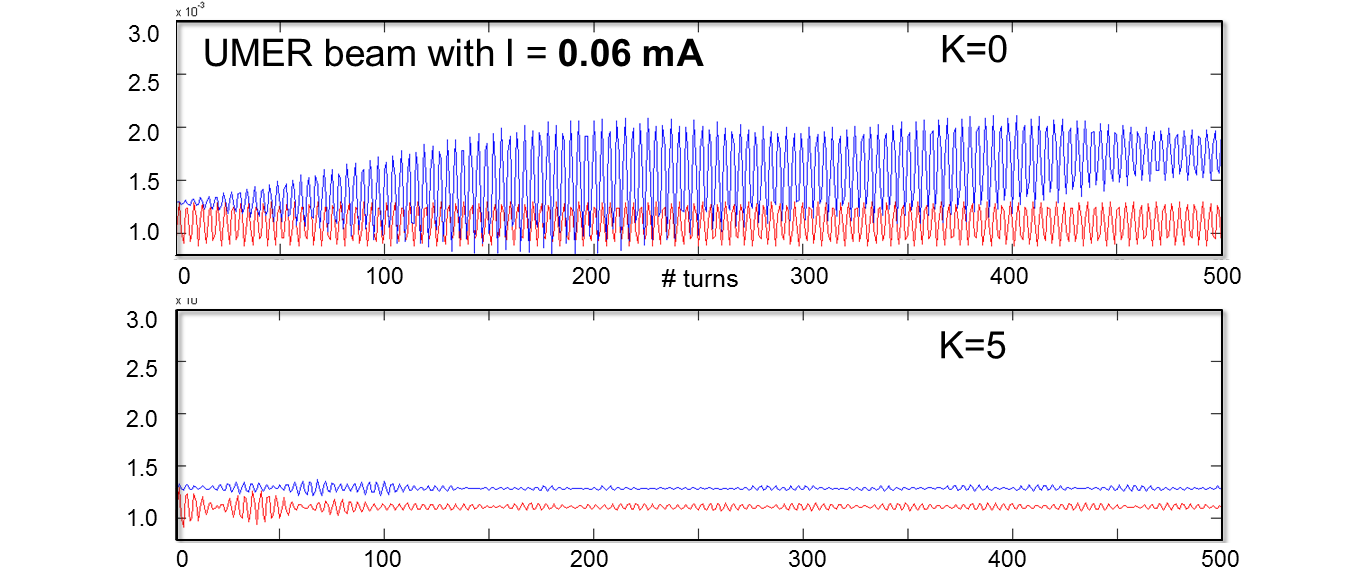
\includegraphics[width=\textwidth]{5.figures/space-charge/60microAmp_rms.png}
}\label{fig:halo-rms-60muA}
\subfigure[]{
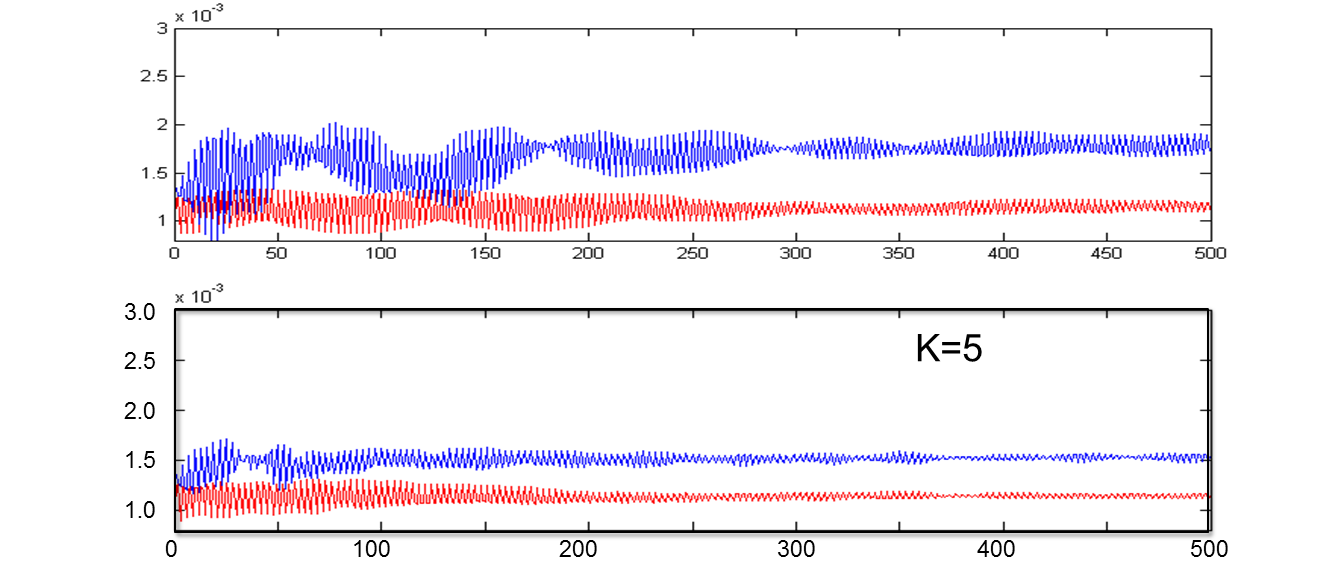
\includegraphics[width=\textwidth]{5.figures/space-charge/pencilbeamAmp_rms.png}
}\label{fig:halo-rms-pencil}
\caption{}
\label{fig:halo-rms}
\end{figure}

\begin{figure}[]
\centering
\subfigure[]{
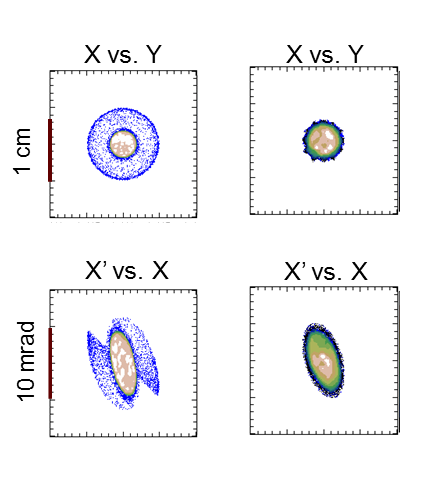
\includegraphics[width=0.4\textwidth]{5.figures/space-charge/60microAmp_snap.png}
}\label{fig:halo-snap-60muA}
\subfigure[]{
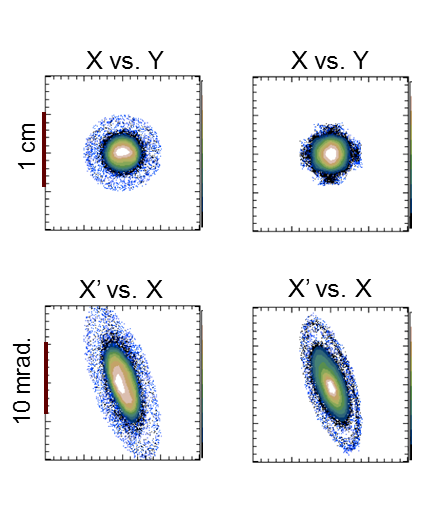
\includegraphics[width=0.4\textwidth]{5.figures/space-charge/pencilbeamAmp_snap.png}
}\label{fig:halo-snap-pencil}
\caption{}
\label{fig:halo-snap}
\end{figure}

%%%%%%%%%%%%%%%%%%%%%%%%%%%%%%%%%%%%%%%%%%%%%%%%%%%%%%%%%%%%%%%%%%%%%%%%%%%%%%%%%%%%%%%%%%%%%%%%%%%%%%%%%%%%%%%%%%%%%%%%%%
%% from AAC14
%%%%%%%%%%%%%%%%%%%%%%%%%%%%%%%%%%%%%%%%%%%%%%%%%%%%%%%%%%%%%%%%%%%%%%%%%%%%%%%%%%%%%%%%%%%%%%%%%%%%%%%%%%%%%%%%%%%%%%%%%%
Initial particle distributions are based on the core/pre-halo method, used by S.D. Webb \cite{Webb2013},\cite{WebbIPAC2013} to demonstrate nonlinear decoherence of mismatched core oscillations that leads to fast suppression of halo formation. In this approach, the beam is modeled in two populations: a mismatched KV core and a matched ‘pre-halo’ observer distribution. The core is initialized with a 30% breathing mode mismatch. With no external nonlinear fields, the pre-halo population is very quickly excited to large amplitudes. 

Simulations were run at the two lowest-current UMER operating points: 6.0 mA and 0.6 mA ‘pencil beam’. While both configurations experienced reduced halo growth with applied octupole fields, the relative effect when compared to the linear cases was diminished in the presence of space charge. Even the 0.6 mA beam suffers from significant space charge tune spread, with an incoherent tune depression of 0.85 in the standard UMER lattice. Additional simulations with a 60 μA beam, which has tune depression of 0.96, show a much more dramatic effect, as shown in Fig. 4. A 60 μA, or “negligible space charge,” beam may be more desirable for halo mitigation experiments and is closer to the regime occupied by existing intense accelerators and storage rings. 




 %%todo: cite Radiasoft 2017 IOTA meeting presentation?

 

  
 \section{Experimental Design}
 \subsection{Channel Design}
 
\begin{figure}[]
\centering
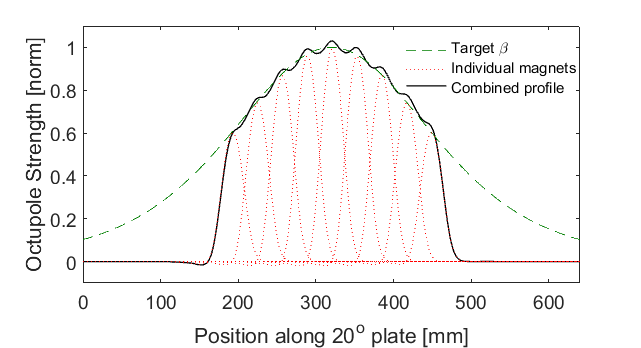
\includegraphics[width=\textwidth]{5.figures/long_channel_N9_cleanedup.png}   
\caption{Composite octupole channel made of over-lapping, evenly-spaced discrete short PCB octupoles.}
\label{fig:octchannel}
\end{figure}  



\section{Matching UMER for nonlinear experiments}
\subsection{0-current lattice solution in Elegant}
\subsubsection{Sensitivity to quadrupole errors}
\subsection{Effect of edge-focusing}
\subsection{Empirical matching}
\subsubsection{Chromaticity and dispersion}





\section{Full ring simulation of octupole lattice}
\subsection{Frequency Map Analysis in Elegant}
\subsection{WARP (time-permitting)}

